\chapter{Estudo dos Dados}
\label{cap:estudodados}


\section{Preparo dos Dados}


Os dados estão distribuícdos em colunas com diversas propriedades analisadas em
laboratório de cada lote retirado da fábrica. Existem diversas planilhas para
lotes retirados de diversas partes do processo de fabricação. Devido a dificuldades logísticas de se casar um
mesmo lote de cimento em diferentes partes do processo (e.g. o mesmo lote ao
sair do forno e depois de finalizado e pronto para vender), estudos serão feitos apenas para os dados de
\textit{expedição de cimento}. 

Segue uma breve definição de cada coluna dos dados de Expedição de Cimento: \\

\begin{itemize}
\item (i) Porcentagens relacionadas a Composição Química: AL\textsubscript{2}O\textsubscript{3}, SIO\textsubscript{2}, MGO, RICARB, P\textsubscript{2}O\textsubscript{5} and FE\textsubscript{2}O\textsubscript{3}
\item (ii) Porcentagem de massa de água em relação ao cimento: AGP
\item (iii) Tempo (em segundos) que o material demora para começar e terminar a endurecer, respectivamente: IP, FP
\item (iv) Finura Blaine, medido em centimetros quadrados por grama ($Cm^{2}/g)$: SBL
\item (v) As medidas de CSC respectivamente 3, 7 e 28 dias após a expedição do lote de cimento: RC3, RC7, RC28
\end{itemize}


Os dados de expedição de cimento são anotados aproximadamente por dia, possuindo 2520
entradas para 3650 dias distintos. Ou seja, existem dias sem dados presentes. O
período contemplado pela planilha de dados vai do dia 02/01/2008 até o dia 29/12/2018.

\subsection{Dados faltantes}

Embora tenhamos uma quantidade razoável de dias com dados presentes, esses muitas vezes não possuem algum valor de alguma coluna.
A seguir vemos para os dados de Expedição de Cimento, para cada uma de suas colunas, a porcentagem de dados presentes. 


\begin{figure}[H]
  \centering
  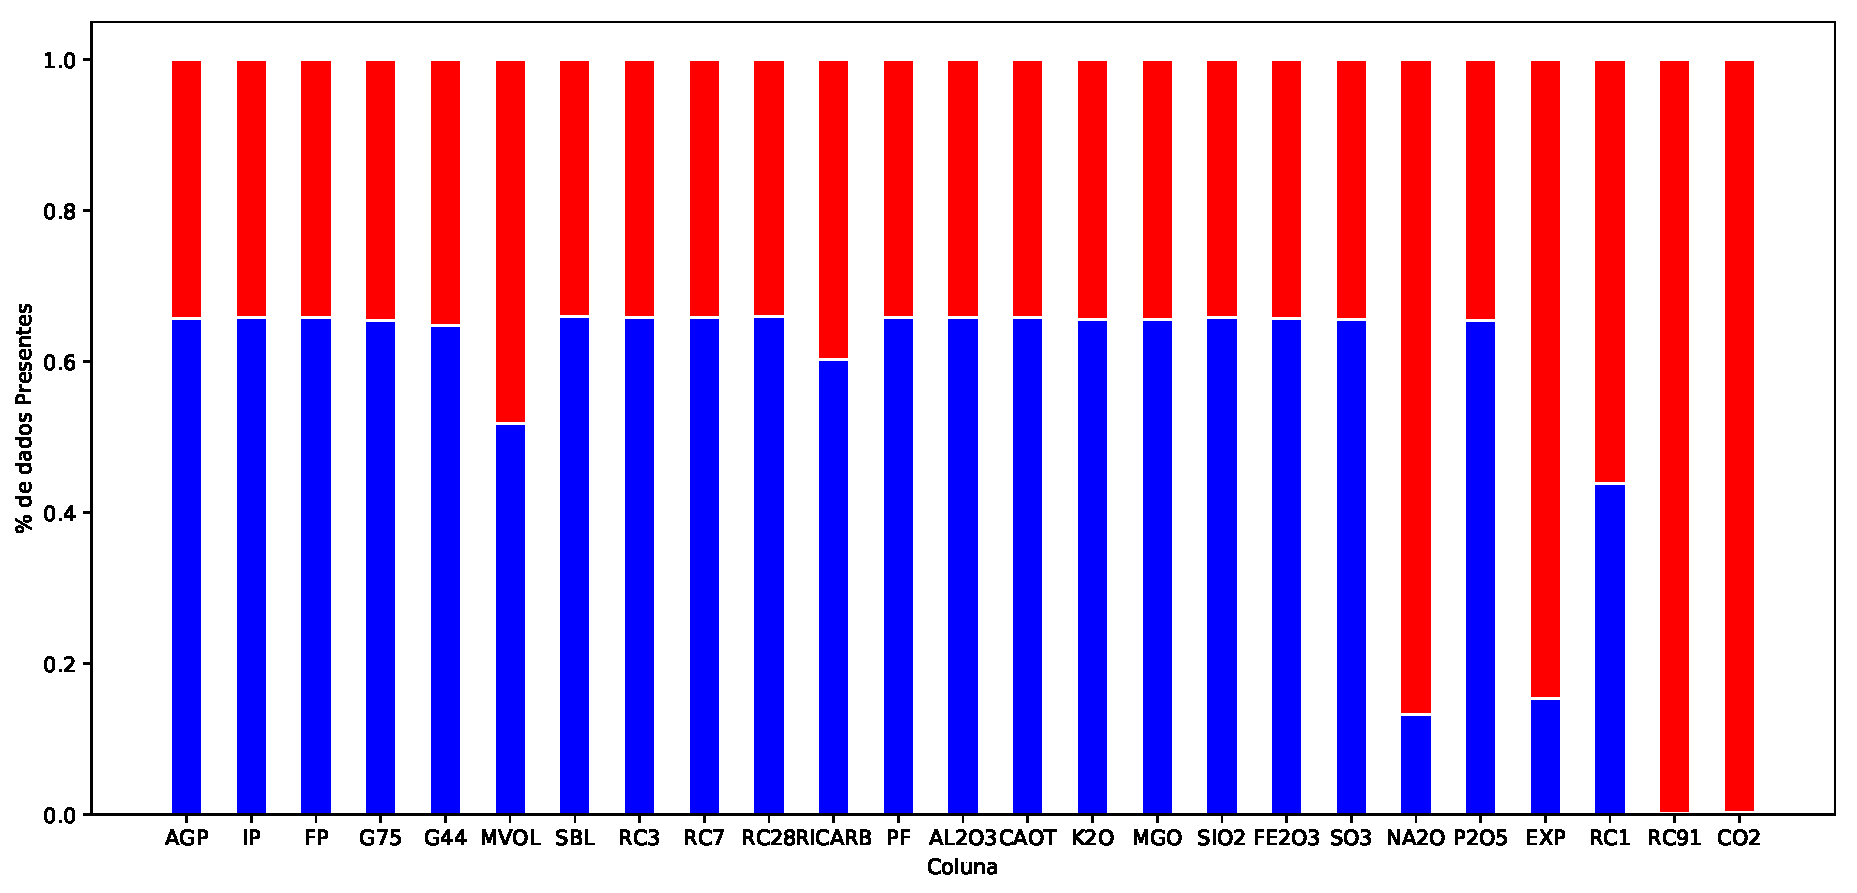
\includegraphics[width=0.9\columnwidth]{slides_dados_pct.pdf}
  \caption{Porcentagem de dados faltantes por Coluna para dados de Expedição de Cimento}
  \label{fig:dadosfalta}
\end{figure}


\section{Reamostragem dos dados}

Uma dos requisitos dos dados assumidos pelos modelos temporais, é que os mesmos
são espaçados regularmente pelo incremento de tempo escolhido, sem lacunas.
Portanto, os dados foram modificados para que entradas anotadas no mesmo dia
sejam unificadas em um único dia. Além disso, para dias no intervalo de tempo
estudado que não possuam entradas, foram criadas entradas com valores
artificiais que não perturbem a distribuição dos dados, e.g. os valores da
última entrada válida são copiados para frente até que se possua um novo valor.

A Figura \ref{fig:reamos} mostra como os dados estavam antes da reamostragem
para que eles se tornem diários: 

\begin{figure}[H]
  \centering
  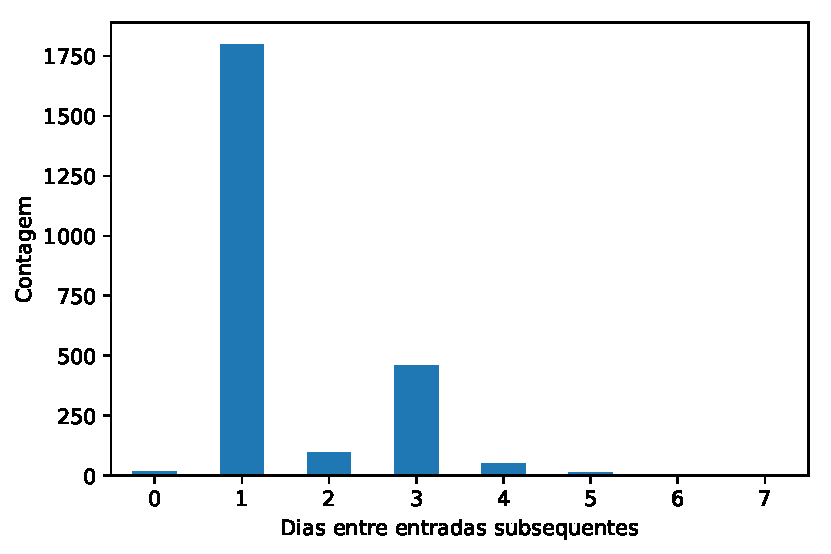
\includegraphics[width=0.5\columnwidth]{slides_dados_antes_resample.pdf}
  \caption{Distribuição das distâncias entre entradas subsequentes dos dados de Expedição de Cimento, antes da reamostragem.}
  \label{fig:reamos}
\end{figure}



\section{Testes de Sazonalidade}

Diversas publicações recentes estudam a eficácia de modelos de Deep Learning
para predição de séries temporais, como consumo de energia elétrica
\citep{lstmbr}. Os dados estudados nesse documento são séries temporais dado que
são indexados pelo tempo, porém, resta analisar características temporais desses
dados. Como exemplo, \cite{lstmbr} usaram a informação do mês atual como
parâmetro para prever o consumo de energia elétrica. Dados que não possuem nenhuma característica temporal (i.e. a ordem não importa) seriam por exemplo provenientes de um estudo do salário recebido por uma amostra da população dados fatores como gênero, escolaridade e idade. No primeiro exemplo temos um caso de \textbf{sazonalidade} nos dados, algo que pode ser analisado em séries temporais com testes de análise espectral e auto-correlação. Para os dados desse problema, iremos testar a sazonalidade dos preditores de dureza do cimento.

\subsection{Análise Espectral}

Uma maneira de testar sazonalidade de dados indexados temporalmente é usar a
técnica de Transformada de Fourier \citep{spec}, onde podemos estudar quais
frequências dentro de um espectro podem ser usadas para decompor um sinal (i.e.
nossos dados). Para essa análise usamos os índices de dureza contidos nos dados
de expedição, de 2008 até 2014 e descartamos a parte imaginária da análise já
que nossos dados não possuem parte complexa \citep{spec}. Seguem os resultados:

\begin{figure}[H]
\centering
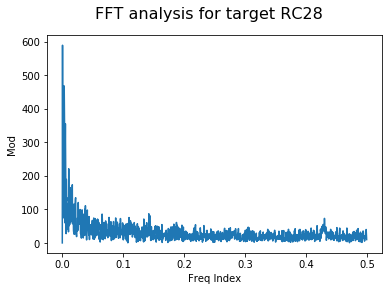
\includegraphics[width=0.9\columnwidth]{FFT_RC28.png}
\caption{Análise Espectral para preditor RC28}
\end{figure}


Podemos notar que a "energia" do sinal não possui picos em nenhuma frequência além da frequência zero, que seria a potência média do sinal, ou seja, uma componente que não depende do tempo. Então, afirmamos que esses dados não possuem sazonalidade mensal ou anual. O que significa que a média e a variância desses indicadores não possuem tendências e.g. alguma mudança similar todo mês de Janeiro.


\section{Correlação entre Colunas}

Vamos analisar agora a \textit{correlação} entre colunas dos dados de expedição
de cimento. Usaremos sempre a \textit{correlação de Pearson} para os cálculos.
\\
Sejam dois vetores de
dados $\{x_1,x_2, \dots , x_n\}$ e $\{y_1,y_2, \dots , y_n\}$, ambos com $n$ entradas. A correlação de Pearson $r$ é calculada
por meio da seguinte fórmula, onde $\overline{x}$ denota a média amostral do
vetor $X$: \\



\[ r = \frac{{}\sum_{i=1}^{n} (x_i - \overline{x})(y_i - \overline{y})}
{\sqrt{\sum_{i=1}^{n} (x_i - \overline{x})^2(y_i - \overline{y})^2}} \] 


\bigskip


A Tabela~\ref{corr3728} mostra correlação entre os índices de resistência dos dados de
expedição de cimento. \\

\begin{table}[H]
\centering
\begin{tabular}{l|lll}
\cline{2-4}
\textbf{}                  & \multicolumn{1}{l|}{RC3} & \multicolumn{1}{l|}{RC7} & \multicolumn{1}{l|}{RC28} \\ \hline
\multicolumn{1}{|l|}{RC3}  & 1                        & 0.734201                 & 0.388973                  \\ \cline{1-1}
\multicolumn{1}{|l|}{RC7}  & 0.734201                 & 1                        & 0.484725                  \\ \cline{1-1}
\multicolumn{1}{|l|}{RC28} & 0.388973                 & 0.484725                 & 1                         \\ \cline{1-1}
\end{tabular}
\caption{Correlação entre Índices de Resistência dos dados de
  Expedição de Cimento}
\label{corr3728}
\end{table}


\section{Normalização}

Os dados foram normalizados pelo método min-max. Essa técnica foi escolhida pelo
fato da distribuição dos dados não ser normal.

Seja um vetor $X$ com $N$ entradas. Podemos normaliza-lo por esse método usando a
seguinte transformação:


\[
x^*_{n} = ( x_n - Min(X))/(Max(X) - Min(X)) 
\]

$Min(X)$  e $Max(X)$ são constantes que devem ser guardadas para posterior
desnormalização do vetor.





%%% Local Variables:
%%% mode: latex
%%% TeX-master: "../quali"
%%% End:
